\documentclass{book}
\usepackage[a4paper,top=2.5cm,bottom=2.5cm,left=2.5cm,right=2.5cm]{geometry}
\usepackage{makeidx}
\usepackage{natbib}
\usepackage{graphicx}
\usepackage{multicol}
\usepackage{float}
\usepackage{listings}
\usepackage{color}
\usepackage{ifthen}
\usepackage[table]{xcolor}
\usepackage{textcomp}
\usepackage{alltt}
\usepackage{ifpdf}
\ifpdf
\usepackage[pdftex,
            pagebackref=true,
            colorlinks=true,
            linkcolor=blue,
            unicode
           ]{hyperref}
\else
\usepackage[ps2pdf,
            pagebackref=true,
            colorlinks=true,
            linkcolor=blue,
            unicode
           ]{hyperref}
\usepackage{pspicture}
\fi
\usepackage[utf8]{inputenc}
\usepackage{mathptmx}
\usepackage[scaled=.90]{helvet}
\usepackage{courier}
\usepackage{sectsty}
\usepackage{amssymb}
\usepackage[titles]{tocloft}
\usepackage{doxygen}
\lstset{language=C++,inputencoding=utf8,basicstyle=\footnotesize,breaklines=true,breakatwhitespace=true,tabsize=4,numbers=left }
\makeindex
\setcounter{tocdepth}{3}
\renewcommand{\footrulewidth}{0.4pt}
\renewcommand{\familydefault}{\sfdefault}
\hfuzz=15pt
\setlength{\emergencystretch}{15pt}
\hbadness=750
\tolerance=750
\begin{document}
\hypersetup{pageanchor=false,citecolor=blue}
\begin{titlepage}
\vspace*{7cm}
\begin{center}
{\Large D\-S\-A\-A\-D\-O\-O\-P \\[1ex]\large 1 }\\
\vspace*{1cm}
{\large Generated by Doxygen 1.8.3.1}\\
\vspace*{0.5cm}
{\small Fri Apr 19 2013 23:37:05}\\
\end{center}
\end{titlepage}
\clearemptydoublepage
\pagenumbering{roman}
\tableofcontents
\clearemptydoublepage
\pagenumbering{arabic}
\hypersetup{pageanchor=true,citecolor=blue}
\chapter{S\-O\-C\-C\-E\-R T\-E\-A\-M T\-R\-A\-C\-K\-E\-R v1.0}
\label{index}\hypertarget{index}{}\hypertarget{index_intro}{}\section{System Introduction}\label{index_intro}
This system creates a Pioneer Car Radio. It inherits from the Am\-Fm\-Radio class and models a real life radio. This program tests whether or not all functions are working.



 \hypertarget{index_knownBugs}{}\section{Known Issues and Limitations}\label{index_knownBugs}
\begin{DoxyRefDesc}{Bug}
\item[\hyperlink{bug__bug000001}{Bug}]\mbox{[}optionally include known bugs and limitations within the project here\mbox{]}
\begin{DoxyItemize}
\item B\-U\-G \-: Volume does not increment properly 
\end{DoxyItemize}\end{DoxyRefDesc}




 \hypertarget{index_version}{}\section{Current version of the Some Project \-:}\label{index_version}

\begin{DoxyItemize}
\item \begin{DoxyAuthor}{Author}
Mike Sadowski 
\end{DoxyAuthor}

\item \begin{DoxyVersion}{Version}
1.\-00.\-00 
\end{DoxyVersion}

\item \begin{DoxyDate}{Date}
March 16th, 2013 
\end{DoxyDate}

\end{DoxyItemize}
\chapter{Todo List}
\label{todo}
\hypertarget{todo}{}

\begin{DoxyRefList}
\item[\label{todo__todo000001}%
\hypertarget{todo__todo000001}{}%
page \hyperlink{index}{S\-O\-C\-C\-E\-R T\-E\-A\-M T\-R\-A\-C\-K\-E\-R v1.0} ]Move functions into classes 

Create test module \#3
\end{DoxyRefList}
\chapter{Hierarchical Index}
\section{Class Hierarchy}
This inheritance list is sorted roughly, but not completely, alphabetically\-:\begin{DoxyCompactList}
\item \contentsline{section}{Amfm\-Radio}{\pageref{class_amfm_radio}}{}
\begin{DoxyCompactList}
\item \contentsline{section}{Pioneer\-Car\-Radio}{\pageref{class_pioneer_car_radio}}{}
\end{DoxyCompactList}
\item \contentsline{section}{Freqs}{\pageref{struct_freqs}}{}
\end{DoxyCompactList}

\chapter{Class Index}
\section{Class List}
Here are the classes, structs, unions and interfaces with brief descriptions\-:\begin{DoxyCompactList}
\item\contentsline{section}{\hyperlink{class_amfm_radio}{Amfm\-Radio} \\*{\bfseries This class models an A\-M/\-F\-M radio} }{\pageref{class_amfm_radio}}{}
\item\contentsline{section}{\hyperlink{struct_freqs}{Freqs} }{\pageref{struct_freqs}}{}
\item\contentsline{section}{\hyperlink{class_pioneer_car_radio}{Pioneer\-Car\-Radio} \\*{\bfseries This class is an Am\-Fm\-Radio, that represents a Pioneer Car Radio in real life} }{\pageref{class_pioneer_car_radio}}{}
\end{DoxyCompactList}

\chapter{File Index}
\section{File List}
Here is a list of all files with brief descriptions\-:\begin{DoxyCompactList}
\item\contentsline{section}{\hyperlink{_d_oxygen_main_project_page_8h}{D\-Oxygen\-Main\-Project\-Page.\-h} }{\pageref{_d_oxygen_main_project_page_8h}}{}
\item\contentsline{section}{\hyperlink{_management_8cpp}{Management.\-cpp} }{\pageref{_management_8cpp}}{}
\item\contentsline{section}{\hyperlink{_management_8h}{Management.\-h} }{\pageref{_management_8h}}{}
\item\contentsline{section}{\hyperlink{project_8cpp}{project.\-cpp} }{\pageref{project_8cpp}}{}
\item\contentsline{section}{\hyperlink{_team_8cpp}{Team.\-cpp} }{\pageref{_team_8cpp}}{}
\item\contentsline{section}{\hyperlink{_team_8h}{Team.\-h} }{\pageref{_team_8h}}{}
\item\contentsline{section}{\hyperlink{unit_test_driver1_8cpp}{unit\-Test\-Driver1.\-cpp} }{\pageref{unit_test_driver1_8cpp}}{}
\item\contentsline{section}{\hyperlink{unit_test_driver2_8cpp}{unit\-Test\-Driver2.\-cpp} }{\pageref{unit_test_driver2_8cpp}}{}
\item\contentsline{section}{\hyperlink{unit_test_driver3_8cpp}{unit\-Test\-Driver3.\-cpp} }{\pageref{unit_test_driver3_8cpp}}{}
\end{DoxyCompactList}

\chapter{Class Documentation}
\hypertarget{class_management}{\section{Management Class Reference}
\label{class_management}\index{Management@{Management}}
}


{\bfseries Brief Description} -\/ Class representing the management/staff of a soccer team  




{\ttfamily \#include $<$Management.\-h$>$}

Inheritance diagram for Management\-:\begin{figure}[H]
\begin{center}
\leavevmode
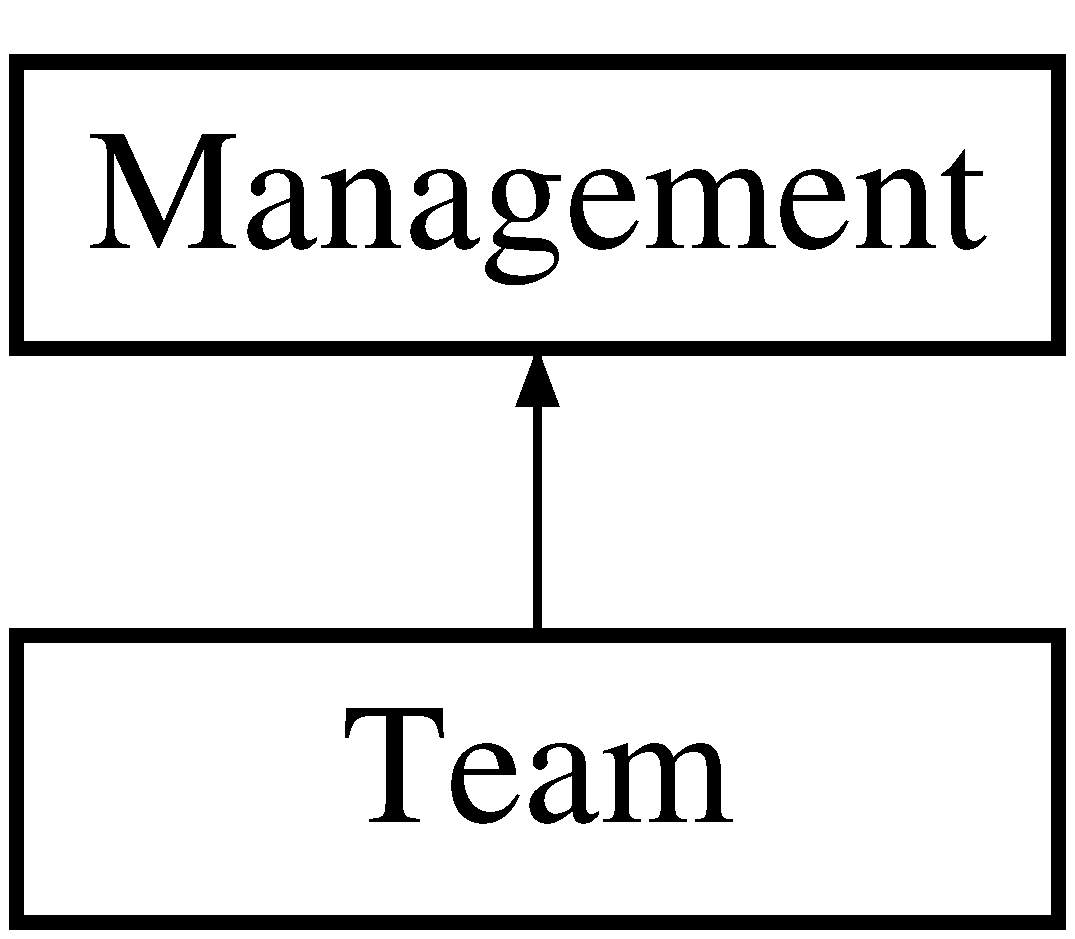
\includegraphics[height=2.000000cm]{class_management}
\end{center}
\end{figure}
\subsection*{Public Member Functions}
\begin{DoxyCompactItemize}
\item 
\hyperlink{class_management_a257178d02f42de0901c3841449ff8bb1}{Management} (void)
\begin{DoxyCompactList}\small\item\em {\bfseries Brief Description} -\/ Constructor \end{DoxyCompactList}\item 
\hyperlink{class_management_a5e386c7700d6dcc0c1728be3a551b918}{$\sim$\-Management} (void)
\begin{DoxyCompactList}\small\item\em {\bfseries Brief Description} -\/ Destructor \end{DoxyCompactList}\item 
const string \hyperlink{class_management_ad2d09a9d74ff2e5fbea54efcd76577a0}{Get\-Team\-Name} (void)
\begin{DoxyCompactList}\small\item\em {\bfseries Brief Description} -\/ Accessor \end{DoxyCompactList}\item 
const string \hyperlink{class_management_a6c6b73df06dc1c04f24d1c5acf94cad4}{Get\-Head\-Coach} (void)
\begin{DoxyCompactList}\small\item\em {\bfseries Brief Description} -\/ Accessor \end{DoxyCompactList}\item 
const string \hyperlink{class_management_a4f35b2aa96601b31e78aaf153300b41d}{Get\-Assistant\-Coach} (void)
\begin{DoxyCompactList}\small\item\em {\bfseries Brief Description} -\/ Accessor \end{DoxyCompactList}\item 
bool \hyperlink{class_management_af1e575b19ed269369eeef2de5719dec8}{Set\-Team\-Name} (string new\-Team\-Name)
\begin{DoxyCompactList}\small\item\em {\bfseries Brief Description} -\/ Mutator \end{DoxyCompactList}\item 
bool \hyperlink{class_management_a678515f513782f5516ac5b1c653a2456}{Set\-Head\-Coach} (string new\-Head\-Coach)
\begin{DoxyCompactList}\small\item\em {\bfseries Brief Description} -\/ Mutator \end{DoxyCompactList}\item 
bool \hyperlink{class_management_a5d4d5d0bc503032c9c26ce15c62bbec8}{Set\-Assistant\-Coach} (string new\-Assistant\-Coach)
\begin{DoxyCompactList}\small\item\em {\bfseries Brief Description} -\/ Mutator \end{DoxyCompactList}\item 
bool \hyperlink{class_management_a4679efc7274b90fa967dc1349d247093}{Check\-Characters\-Of\-String} (string my\-String)
\begin{DoxyCompactList}\small\item\em {\bfseries Brief Description} -\/ Validator Function \end{DoxyCompactList}\end{DoxyCompactItemize}
\subsection*{Private Attributes}
\begin{DoxyCompactItemize}
\item 
string \hyperlink{class_management_a78344be52d9cb5025226b4939e562901}{team\-Name}
\item 
string \hyperlink{class_management_aaec7a4d4d85085cc58237f23b29648bc}{head\-Coach}
\item 
string \hyperlink{class_management_a0255211caa5f03eaf86491d069e36921}{assistant\-Coach}
\end{DoxyCompactItemize}


\subsection{Detailed Description}
{\bfseries Brief Description} -\/ Class representing the management/staff of a soccer team 

This class replicates the management and staff of a soccer team. It contains the name of the head coach, assistant coach, and what the name of the soccer team is. It also contains a function that is used to verify all names of players/coaches on the team, and checks if the string contains characters that are not supposed to be a part of the person's name.


\begin{DoxyItemize}
\item class constants\-:
\begin{DoxyItemize}
\item T\-E\-A\-M\-N\-A\-M\-E\-A\-T\-T\-R\-I\-B\-U\-T\-E\-N\-U\-M indicates a change to the team name is wanted
\item H\-E\-A\-D\-C\-O\-A\-C\-H\-A\-T\-T\-R\-I\-B\-U\-T\-E\-N\-U\-M indicates a change to the head coach name is wanted
\item A\-S\-S\-I\-S\-T\-A\-N\-T\-C\-O\-A\-C\-H\-A\-T\-T\-R\-I\-B\-U\-T\-E\-N\-U\-M indicates a change to the assitant coach name is wanted
\item S\-T\-A\-R\-T\-E\-R\-A\-T\-R\-R\-I\-B\-U\-T\-E\-N\-U\-M indicates a change to the starters is wanted
\item B\-A\-C\-K\-U\-P\-A\-T\-R\-R\-I\-B\-U\-T\-E\-N\-U\-M indicates a change to the backups is wanted
\item A\-L\-L\-A\-T\-T\-R\-I\-B\-U\-T\-E\-S indicates a change to the team name is wanted
\item A\-R\-R\-A\-Y\-S\-I\-Z\-E is the max array size
\item M\-A\-X\-S\-T\-A\-R\-T\-E\-R\-S max amount of starters allowed (11)
\item M\-A\-X\-B\-A\-C\-K\-U\-P\-S max amount of backups allowed (5)
\item M\-A\-X\-L\-E\-N\-G\-T\-H max length of user input (255 characters)
\item B\-U\-F\-F\-E\-R\-S\-I\-Z\-E max length of a buffer (1000 characters)
\end{DoxyItemize}
\end{DoxyItemize}


\begin{DoxyItemize}
\item class data members (attributes)\-:
\begin{DoxyItemize}
\item string team\-Name; contains the name of the team
\item string head\-Coach; contains the name of the head coach
\item string assistant\-Coach; contains the name of the assistant coach
\end{DoxyItemize}
\end{DoxyItemize}

\begin{DoxyAuthor}{Author}
{\itshape Mike Sadowski} 
\end{DoxyAuthor}


\subsection{Constructor \& Destructor Documentation}
\hypertarget{class_management_a257178d02f42de0901c3841449ff8bb1}{\index{Management@{Management}!Management@{Management}}
\index{Management@{Management}!Management@{Management}}
\subsubsection[{Management}]{\setlength{\rightskip}{0pt plus 5cm}Management\-::\-Management (
\begin{DoxyParamCaption}
\item[{void}]{}
\end{DoxyParamCaption}
)}}\label{class_management_a257178d02f42de0901c3841449ff8bb1}


{\bfseries Brief Description} -\/ Constructor 

Constructor for the \hyperlink{class_management}{Management} class. Initializes the team\-Name, head\-Coach, assistant\-Coach strings to equal \char`\"{}\-N\-O\-T\-S\-E\-T\char`\"{}

\begin{DoxyReturn}{Returns}
nothing 
\end{DoxyReturn}
\hypertarget{class_management_a5e386c7700d6dcc0c1728be3a551b918}{\index{Management@{Management}!$\sim$\-Management@{$\sim$\-Management}}
\index{$\sim$\-Management@{$\sim$\-Management}!Management@{Management}}
\subsubsection[{$\sim$\-Management}]{\setlength{\rightskip}{0pt plus 5cm}Management\-::$\sim$\-Management (
\begin{DoxyParamCaption}
\item[{void}]{}
\end{DoxyParamCaption}
)}}\label{class_management_a5e386c7700d6dcc0c1728be3a551b918}


{\bfseries Brief Description} -\/ Destructor 

This is the destructor for the \hyperlink{class_management}{Management} class

\begin{DoxyReturn}{Returns}
nothing 
\end{DoxyReturn}


\subsection{Member Function Documentation}
\hypertarget{class_management_a4679efc7274b90fa967dc1349d247093}{\index{Management@{Management}!Check\-Characters\-Of\-String@{Check\-Characters\-Of\-String}}
\index{Check\-Characters\-Of\-String@{Check\-Characters\-Of\-String}!Management@{Management}}
\subsubsection[{Check\-Characters\-Of\-String}]{\setlength{\rightskip}{0pt plus 5cm}bool Management\-::\-Check\-Characters\-Of\-String (
\begin{DoxyParamCaption}
\item[{string}]{my\-String}
\end{DoxyParamCaption}
)}}\label{class_management_a4679efc7274b90fa967dc1349d247093}


{\bfseries Brief Description} -\/ Validator Function 

This function iterates through an array of available characters, and determines if a string passed in contains a character that is not allowed.

\begin{DoxyReturn}{Returns}
True/\-False if string passed the test 
\end{DoxyReturn}
\hypertarget{class_management_a4f35b2aa96601b31e78aaf153300b41d}{\index{Management@{Management}!Get\-Assistant\-Coach@{Get\-Assistant\-Coach}}
\index{Get\-Assistant\-Coach@{Get\-Assistant\-Coach}!Management@{Management}}
\subsubsection[{Get\-Assistant\-Coach}]{\setlength{\rightskip}{0pt plus 5cm}const string Management\-::\-Get\-Assistant\-Coach (
\begin{DoxyParamCaption}
\item[{void}]{}
\end{DoxyParamCaption}
)}}\label{class_management_a4f35b2aa96601b31e78aaf153300b41d}


{\bfseries Brief Description} -\/ Accessor 

This is the Accessor for the \hyperlink{class_management}{Management} class's variable\-: assistant\-Coach

\begin{DoxyReturn}{Returns}
assistant\-Coach (string) 
\end{DoxyReturn}
\hypertarget{class_management_a6c6b73df06dc1c04f24d1c5acf94cad4}{\index{Management@{Management}!Get\-Head\-Coach@{Get\-Head\-Coach}}
\index{Get\-Head\-Coach@{Get\-Head\-Coach}!Management@{Management}}
\subsubsection[{Get\-Head\-Coach}]{\setlength{\rightskip}{0pt plus 5cm}const string Management\-::\-Get\-Head\-Coach (
\begin{DoxyParamCaption}
\item[{void}]{}
\end{DoxyParamCaption}
)}}\label{class_management_a6c6b73df06dc1c04f24d1c5acf94cad4}


{\bfseries Brief Description} -\/ Accessor 

This is the Accessor for the \hyperlink{class_management}{Management} class's variable\-: head\-Coach

\begin{DoxyReturn}{Returns}
head\-Coach (string) 
\end{DoxyReturn}
\hypertarget{class_management_ad2d09a9d74ff2e5fbea54efcd76577a0}{\index{Management@{Management}!Get\-Team\-Name@{Get\-Team\-Name}}
\index{Get\-Team\-Name@{Get\-Team\-Name}!Management@{Management}}
\subsubsection[{Get\-Team\-Name}]{\setlength{\rightskip}{0pt plus 5cm}const string Management\-::\-Get\-Team\-Name (
\begin{DoxyParamCaption}
\item[{void}]{}
\end{DoxyParamCaption}
)}}\label{class_management_ad2d09a9d74ff2e5fbea54efcd76577a0}


{\bfseries Brief Description} -\/ Accessor 

This is the Accessor for the \hyperlink{class_management}{Management} class's variable\-: team\-Name

\begin{DoxyReturn}{Returns}
team\-Name (string) 
\end{DoxyReturn}
\hypertarget{class_management_a5d4d5d0bc503032c9c26ce15c62bbec8}{\index{Management@{Management}!Set\-Assistant\-Coach@{Set\-Assistant\-Coach}}
\index{Set\-Assistant\-Coach@{Set\-Assistant\-Coach}!Management@{Management}}
\subsubsection[{Set\-Assistant\-Coach}]{\setlength{\rightskip}{0pt plus 5cm}bool Management\-::\-Set\-Assistant\-Coach (
\begin{DoxyParamCaption}
\item[{string}]{new\-Assistant\-Coach}
\end{DoxyParamCaption}
)}}\label{class_management_a5d4d5d0bc503032c9c26ce15c62bbec8}


{\bfseries Brief Description} -\/ Mutator 

This is the Mutator for the \hyperlink{class_management}{Management} class's variable\-: assistant\-Coach It also validates all incoming data.

\begin{DoxyReturn}{Returns}
True/\-False if member was set or not 
\end{DoxyReturn}
\hypertarget{class_management_a678515f513782f5516ac5b1c653a2456}{\index{Management@{Management}!Set\-Head\-Coach@{Set\-Head\-Coach}}
\index{Set\-Head\-Coach@{Set\-Head\-Coach}!Management@{Management}}
\subsubsection[{Set\-Head\-Coach}]{\setlength{\rightskip}{0pt plus 5cm}bool Management\-::\-Set\-Head\-Coach (
\begin{DoxyParamCaption}
\item[{string}]{new\-Head\-Coach}
\end{DoxyParamCaption}
)}}\label{class_management_a678515f513782f5516ac5b1c653a2456}


{\bfseries Brief Description} -\/ Mutator 

This is the Mutator for the \hyperlink{class_management}{Management} class's variable\-: head\-Coach It also validates all incoming data.

\begin{DoxyReturn}{Returns}
True/\-False if member was set or not 
\end{DoxyReturn}
\hypertarget{class_management_af1e575b19ed269369eeef2de5719dec8}{\index{Management@{Management}!Set\-Team\-Name@{Set\-Team\-Name}}
\index{Set\-Team\-Name@{Set\-Team\-Name}!Management@{Management}}
\subsubsection[{Set\-Team\-Name}]{\setlength{\rightskip}{0pt plus 5cm}bool Management\-::\-Set\-Team\-Name (
\begin{DoxyParamCaption}
\item[{string}]{new\-Team\-Name}
\end{DoxyParamCaption}
)}}\label{class_management_af1e575b19ed269369eeef2de5719dec8}


{\bfseries Brief Description} -\/ Mutator 

This is the Mutator for the \hyperlink{class_management}{Management} class's variable\-: team\-Name It also validates all incoming data.

\begin{DoxyReturn}{Returns}
True/\-False if member was set or not 
\end{DoxyReturn}


\subsection{Member Data Documentation}
\hypertarget{class_management_a0255211caa5f03eaf86491d069e36921}{\index{Management@{Management}!assistant\-Coach@{assistant\-Coach}}
\index{assistant\-Coach@{assistant\-Coach}!Management@{Management}}
\subsubsection[{assistant\-Coach}]{\setlength{\rightskip}{0pt plus 5cm}string Management\-::assistant\-Coach\hspace{0.3cm}{\ttfamily [private]}}}\label{class_management_a0255211caa5f03eaf86491d069e36921}
\hypertarget{class_management_aaec7a4d4d85085cc58237f23b29648bc}{\index{Management@{Management}!head\-Coach@{head\-Coach}}
\index{head\-Coach@{head\-Coach}!Management@{Management}}
\subsubsection[{head\-Coach}]{\setlength{\rightskip}{0pt plus 5cm}string Management\-::head\-Coach\hspace{0.3cm}{\ttfamily [private]}}}\label{class_management_aaec7a4d4d85085cc58237f23b29648bc}
\hypertarget{class_management_a78344be52d9cb5025226b4939e562901}{\index{Management@{Management}!team\-Name@{team\-Name}}
\index{team\-Name@{team\-Name}!Management@{Management}}
\subsubsection[{team\-Name}]{\setlength{\rightskip}{0pt plus 5cm}string Management\-::team\-Name\hspace{0.3cm}{\ttfamily [private]}}}\label{class_management_a78344be52d9cb5025226b4939e562901}


The documentation for this class was generated from the following files\-:\begin{DoxyCompactItemize}
\item 
\hyperlink{_management_8h}{Management.\-h}\item 
\hyperlink{_management_8cpp}{Management.\-cpp}\end{DoxyCompactItemize}

\hypertarget{class_team}{\section{Team Class Reference}
\label{class_team}\index{Team@{Team}}
}


{\bfseries Brief Description} -\/ Class representing the players of a soccer team  




{\ttfamily \#include $<$Team.\-h$>$}

Inheritance diagram for Team\-:\begin{figure}[H]
\begin{center}
\leavevmode
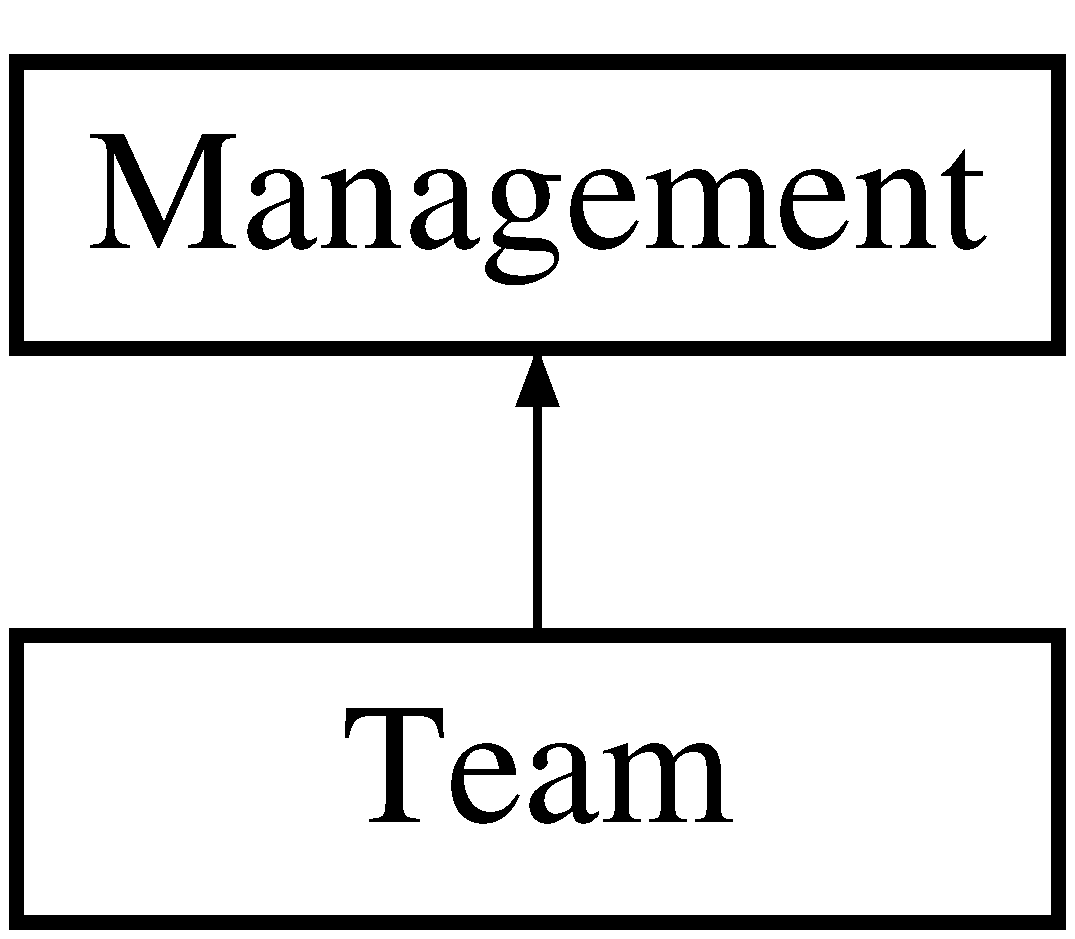
\includegraphics[height=2.000000cm]{class_team}
\end{center}
\end{figure}
\subsection*{Public Member Functions}
\begin{DoxyCompactItemize}
\item 
\hyperlink{class_team_a5c50ce3e6092301c0fa990d924b3827f}{Team} (void)
\begin{DoxyCompactList}\small\item\em {\bfseries Brief Description} -\/ Constructor \end{DoxyCompactList}\item 
\hyperlink{class_team_ad0b24ef1a01a350f03517022070f4d74}{$\sim$\-Team} (void)
\begin{DoxyCompactList}\small\item\em {\bfseries Brief Description} -\/ Destructor \end{DoxyCompactList}\item 
const string $\ast$ \hyperlink{class_team_a18cb95e82e37488b41d3dd001431e8ec}{Get\-Starters} (void)
\begin{DoxyCompactList}\small\item\em {\bfseries Brief Description} -\/ Accessor \end{DoxyCompactList}\item 
const string $\ast$ \hyperlink{class_team_a5b802edf160b74d7428d3ee744d847fb}{Get\-Backups} (void)
\begin{DoxyCompactList}\small\item\em {\bfseries Brief Description} -\/ Accessor \end{DoxyCompactList}\item 
bool $\ast$ \hyperlink{class_team_af808fa3ac89d09c75019f0119f2a7ee1}{Set\-Starters} (const string new\-Starters\mbox{[}$\,$\mbox{]})
\begin{DoxyCompactList}\small\item\em {\bfseries Brief Description} -\/ Mutator \end{DoxyCompactList}\item 
bool $\ast$ \hyperlink{class_team_a74a3662a1280c55934675fa6685c8886}{Set\-Backups} (const string new\-Backups\mbox{[}$\,$\mbox{]})
\begin{DoxyCompactList}\small\item\em {\bfseries Brief Description} -\/ Mutator \end{DoxyCompactList}\item 
void \hyperlink{class_team_a1132a80759e3fcfce0b69d1c8c156016}{Print\-Team\-Info} (void)
\begin{DoxyCompactList}\small\item\em {\bfseries Brief Description} -\/ Prints \hyperlink{class_team}{Team} Information \end{DoxyCompactList}\end{DoxyCompactItemize}
\subsection*{Public Attributes}
\begin{DoxyCompactItemize}
\item 
\hyperlink{class_team}{Team} $\ast$ \hyperlink{class_team_a1d82260b41ee7610a0e36210825a53ea}{next}
\end{DoxyCompactItemize}
\subsection*{Private Attributes}
\begin{DoxyCompactItemize}
\item 
string \hyperlink{class_team_ac3a41d0b7f4013c8643529062bf2c239}{starters} \mbox{[}\hyperlink{_management_8h_a8ad0c96529f809b83cae71c128d9e7af}{M\-A\-X\-S\-T\-A\-R\-T\-E\-R\-S}\mbox{]}
\item 
string \hyperlink{class_team_ad1ef40efc4c39fe0cc34784b872054f7}{backups} \mbox{[}\hyperlink{_management_8h_a14d22215d85e80ff360b526bd4025785}{M\-A\-X\-B\-A\-C\-K\-U\-P\-S}\mbox{]}
\end{DoxyCompactItemize}


\subsection{Detailed Description}
{\bfseries Brief Description} -\/ Class representing the players of a soccer team 

This class replicates the players a soccer team. It contains the name of all 11 starting players, and the 5 backup players. It inherits from the \hyperlink{class_management}{Management} class, which is used to hold the information about the coaches and the team's name, while this class only holds information about the players.


\begin{DoxyItemize}
\item class constants\-:
\begin{DoxyItemize}
\item M\-A\-X\-S\-T\-A\-R\-T\-E\-R\-S max amount of starters allowed (11)
\item M\-A\-X\-B\-A\-C\-K\-U\-P\-S max amount of backups allowed (5)
\item M\-A\-X\-L\-E\-N\-G\-T\-H max length of user input (255 characters)
\item B\-U\-F\-F\-E\-R\-S\-I\-Z\-E max length of a buffer (1000 characters)
\end{DoxyItemize}
\end{DoxyItemize}


\begin{DoxyItemize}
\item class data members (attributes)\-:
\begin{DoxyItemize}
\item string starters\mbox{[}M\-A\-X\-S\-T\-A\-R\-T\-E\-R\-S\mbox{]}; an array of the 11 starting player's names
\item string backups\mbox{[}M\-A\-X\-B\-A\-C\-K\-U\-P\-S\mbox{]}; an array of the 5 backup player's names
\item \hyperlink{class_team}{Team} $\ast$next; a \hyperlink{class_team}{Team} pointer that is used to create a linked list of many objects type \hyperlink{class_team}{Team}
\end{DoxyItemize}
\end{DoxyItemize}

\begin{DoxyAuthor}{Author}
{\itshape Mike Sadowski} 
\end{DoxyAuthor}


\subsection{Constructor \& Destructor Documentation}
\hypertarget{class_team_a5c50ce3e6092301c0fa990d924b3827f}{\index{Team@{Team}!Team@{Team}}
\index{Team@{Team}!Team@{Team}}
\subsubsection[{Team}]{\setlength{\rightskip}{0pt plus 5cm}Team\-::\-Team (
\begin{DoxyParamCaption}
\item[{void}]{}
\end{DoxyParamCaption}
)}}\label{class_team_a5c50ce3e6092301c0fa990d924b3827f}


{\bfseries Brief Description} -\/ Constructor 

Constructor for the \hyperlink{class_team}{Team} class. Initializes the 11 starters and 5 backup player's names as \char`\"{}\-N\-O\-T\-S\-E\-T\char`\"{}

\begin{DoxyReturn}{Returns}
nothing 
\end{DoxyReturn}
\hypertarget{class_team_ad0b24ef1a01a350f03517022070f4d74}{\index{Team@{Team}!$\sim$\-Team@{$\sim$\-Team}}
\index{$\sim$\-Team@{$\sim$\-Team}!Team@{Team}}
\subsubsection[{$\sim$\-Team}]{\setlength{\rightskip}{0pt plus 5cm}Team\-::$\sim$\-Team (
\begin{DoxyParamCaption}
\item[{void}]{}
\end{DoxyParamCaption}
)}}\label{class_team_ad0b24ef1a01a350f03517022070f4d74}


{\bfseries Brief Description} -\/ Destructor 

Destructor for the \hyperlink{class_team}{Team} class.

\begin{DoxyReturn}{Returns}
nothing 
\end{DoxyReturn}


\subsection{Member Function Documentation}
\hypertarget{class_team_a5b802edf160b74d7428d3ee744d847fb}{\index{Team@{Team}!Get\-Backups@{Get\-Backups}}
\index{Get\-Backups@{Get\-Backups}!Team@{Team}}
\subsubsection[{Get\-Backups}]{\setlength{\rightskip}{0pt plus 5cm}const string $\ast$ Team\-::\-Get\-Backups (
\begin{DoxyParamCaption}
\item[{void}]{}
\end{DoxyParamCaption}
)}}\label{class_team_a5b802edf160b74d7428d3ee744d847fb}


{\bfseries Brief Description} -\/ Accessor 

This is the Accessor for the \hyperlink{class_team}{Team} class's variable\-: backups\mbox{[}\mbox{]}

\begin{DoxyReturn}{Returns}
an array of strings (5 backups player's names) 
\end{DoxyReturn}
\hypertarget{class_team_a18cb95e82e37488b41d3dd001431e8ec}{\index{Team@{Team}!Get\-Starters@{Get\-Starters}}
\index{Get\-Starters@{Get\-Starters}!Team@{Team}}
\subsubsection[{Get\-Starters}]{\setlength{\rightskip}{0pt plus 5cm}const string $\ast$ Team\-::\-Get\-Starters (
\begin{DoxyParamCaption}
\item[{void}]{}
\end{DoxyParamCaption}
)}}\label{class_team_a18cb95e82e37488b41d3dd001431e8ec}


{\bfseries Brief Description} -\/ Accessor 

This is the Accessor for the \hyperlink{class_team}{Team} class's variable\-: starters\mbox{[}\mbox{]}

\begin{DoxyReturn}{Returns}
an array of strings (11 starting player's names) 
\end{DoxyReturn}
\hypertarget{class_team_a1132a80759e3fcfce0b69d1c8c156016}{\index{Team@{Team}!Print\-Team\-Info@{Print\-Team\-Info}}
\index{Print\-Team\-Info@{Print\-Team\-Info}!Team@{Team}}
\subsubsection[{Print\-Team\-Info}]{\setlength{\rightskip}{0pt plus 5cm}void Team\-::\-Print\-Team\-Info (
\begin{DoxyParamCaption}
\item[{void}]{}
\end{DoxyParamCaption}
)}}\label{class_team_a1132a80759e3fcfce0b69d1c8c156016}


{\bfseries Brief Description} -\/ Prints \hyperlink{class_team}{Team} Information 

This function prints the teams information in a very neat way. Format\-: \char`\"{}$>$$>$\-Team Name\-: \char`\"{} \char`\"{}$>$$>$\-Head Coach\-: \char`\"{} \char`\"{}$>$$>$\-Assistant Coach\-: \char`\"{} \char`\"{}$>$$>$\-Starting Players\-: \char`\"{} \char`\"{}$>$$>$\-Backup Players\-: \char`\"{} \begin{DoxyReturn}{Returns}
N\-O\-N\-E 
\end{DoxyReturn}
\hypertarget{class_team_a74a3662a1280c55934675fa6685c8886}{\index{Team@{Team}!Set\-Backups@{Set\-Backups}}
\index{Set\-Backups@{Set\-Backups}!Team@{Team}}
\subsubsection[{Set\-Backups}]{\setlength{\rightskip}{0pt plus 5cm}bool $\ast$ Team\-::\-Set\-Backups (
\begin{DoxyParamCaption}
\item[{const string}]{new\-Backups\mbox{[}$\,$\mbox{]}}
\end{DoxyParamCaption}
)}}\label{class_team_a74a3662a1280c55934675fa6685c8886}


{\bfseries Brief Description} -\/ Mutator 

This is the Mutator for the \hyperlink{class_team}{Team} class's variable\-: backups\mbox{[}\mbox{]} It also validates all incoming data.

\begin{DoxyReturn}{Returns}
bool array if the member at that index was set or not 
\end{DoxyReturn}
\hypertarget{class_team_af808fa3ac89d09c75019f0119f2a7ee1}{\index{Team@{Team}!Set\-Starters@{Set\-Starters}}
\index{Set\-Starters@{Set\-Starters}!Team@{Team}}
\subsubsection[{Set\-Starters}]{\setlength{\rightskip}{0pt plus 5cm}bool $\ast$ Team\-::\-Set\-Starters (
\begin{DoxyParamCaption}
\item[{const string}]{new\-Starters\mbox{[}$\,$\mbox{]}}
\end{DoxyParamCaption}
)}}\label{class_team_af808fa3ac89d09c75019f0119f2a7ee1}


{\bfseries Brief Description} -\/ Mutator 

This is the Mutator for the \hyperlink{class_team}{Team} class's variable\-: starters It also validates all incoming data.

\begin{DoxyReturn}{Returns}
bool array if the member at that index was set or not 
\end{DoxyReturn}


\subsection{Member Data Documentation}
\hypertarget{class_team_ad1ef40efc4c39fe0cc34784b872054f7}{\index{Team@{Team}!backups@{backups}}
\index{backups@{backups}!Team@{Team}}
\subsubsection[{backups}]{\setlength{\rightskip}{0pt plus 5cm}string Team\-::backups\mbox{[}{\bf M\-A\-X\-B\-A\-C\-K\-U\-P\-S}\mbox{]}\hspace{0.3cm}{\ttfamily [private]}}}\label{class_team_ad1ef40efc4c39fe0cc34784b872054f7}
\hypertarget{class_team_a1d82260b41ee7610a0e36210825a53ea}{\index{Team@{Team}!next@{next}}
\index{next@{next}!Team@{Team}}
\subsubsection[{next}]{\setlength{\rightskip}{0pt plus 5cm}{\bf Team}$\ast$ Team\-::next}}\label{class_team_a1d82260b41ee7610a0e36210825a53ea}
\hypertarget{class_team_ac3a41d0b7f4013c8643529062bf2c239}{\index{Team@{Team}!starters@{starters}}
\index{starters@{starters}!Team@{Team}}
\subsubsection[{starters}]{\setlength{\rightskip}{0pt plus 5cm}string Team\-::starters\mbox{[}{\bf M\-A\-X\-S\-T\-A\-R\-T\-E\-R\-S}\mbox{]}\hspace{0.3cm}{\ttfamily [private]}}}\label{class_team_ac3a41d0b7f4013c8643529062bf2c239}


The documentation for this class was generated from the following files\-:\begin{DoxyCompactItemize}
\item 
\hyperlink{_team_8h}{Team.\-h}\item 
\hyperlink{_team_8cpp}{Team.\-cpp}\end{DoxyCompactItemize}

\chapter{File Documentation}
\hypertarget{_d_oxygen_main_project_page_8h}{\section{D\-Oxygen\-Main\-Project\-Page.\-h File Reference}
\label{_d_oxygen_main_project_page_8h}\index{D\-Oxygen\-Main\-Project\-Page.\-h@{D\-Oxygen\-Main\-Project\-Page.\-h}}
}

\hypertarget{_management_8cpp}{\section{Management.\-cpp File Reference}
\label{_management_8cpp}\index{Management.\-cpp@{Management.\-cpp}}
}
{\ttfamily \#include \char`\"{}Management.\-h\char`\"{}}\\*

\hypertarget{_management_8h}{\section{Management.\-h File Reference}
\label{_management_8h}\index{Management.\-h@{Management.\-h}}
}
{\ttfamily \#include $<$stdio.\-h$>$}\\*
{\ttfamily \#include $<$stdlib.\-h$>$}\\*
{\ttfamily \#include $<$string$>$}\\*
{\ttfamily \#include $<$string.\-h$>$}\\*
{\ttfamily \#include $<$iostream$>$}\\*
{\ttfamily \#include $<$fstream$>$}\\*
{\ttfamily \#include $<$conio.\-h$>$}\\*
\subsection*{Classes}
\begin{DoxyCompactItemize}
\item 
class \hyperlink{class_management}{Management}
\begin{DoxyCompactList}\small\item\em {\bfseries Brief Description} -\/ Class representing the management/staff of a soccer team \end{DoxyCompactList}\end{DoxyCompactItemize}
\subsection*{Macros}
\begin{DoxyCompactItemize}
\item 
\#define \hyperlink{_management_8h_a78d344caabde729a4559393a0552bf1c}{A\-R\-R\-A\-Y\-S\-I\-Z\-E}~100
\item 
\#define \hyperlink{_management_8h_a8ad0c96529f809b83cae71c128d9e7af}{M\-A\-X\-S\-T\-A\-R\-T\-E\-R\-S}~11
\item 
\#define \hyperlink{_management_8h_a14d22215d85e80ff360b526bd4025785}{M\-A\-X\-B\-A\-C\-K\-U\-P\-S}~5
\item 
\#define \hyperlink{_management_8h_a1dbd686f69551b83691025eaae058539}{M\-A\-X\-L\-E\-N\-G\-T\-H}~255
\item 
\#define \hyperlink{_management_8h_ac3146f1e9227301bb4aa518f4d336cee}{B\-U\-F\-F\-E\-R\-S\-I\-Z\-E}~1000
\item 
\#define \hyperlink{_management_8h_a1b54f93aa5690064ed44274d9a874861}{T\-E\-A\-M\-N\-A\-M\-E\-A\-T\-T\-R\-I\-B\-U\-T\-E\-N\-U\-M}~100
\item 
\#define \hyperlink{_management_8h_a24e7eb459fe5931519647ca6f09a4407}{H\-E\-A\-D\-C\-O\-A\-C\-H\-A\-T\-T\-R\-I\-B\-U\-T\-E\-N\-U\-M}~101
\item 
\#define \hyperlink{_management_8h_a78c40d3a2a47bdc99fdd44e3c9861831}{A\-S\-S\-I\-S\-T\-A\-N\-T\-C\-O\-A\-C\-H\-A\-T\-T\-R\-I\-B\-U\-T\-E\-N\-U\-M}~102
\item 
\#define \hyperlink{_management_8h_ab23087946a76fd96e21d4da71bb3186d}{S\-T\-A\-R\-T\-E\-R\-A\-T\-R\-R\-I\-B\-U\-T\-E\-N\-U\-M}~103
\item 
\#define \hyperlink{_management_8h_a63502d8fea277c0d16041adc6ba06025}{B\-A\-C\-K\-U\-P\-A\-T\-R\-R\-I\-B\-U\-T\-E\-N\-U\-M}~104
\item 
\#define \hyperlink{_management_8h_ab55752e74d379366181a609cc8957941}{A\-L\-L\-A\-T\-T\-R\-I\-B\-U\-T\-E\-S}~105
\end{DoxyCompactItemize}


\subsection{Macro Definition Documentation}
\hypertarget{_management_8h_ab55752e74d379366181a609cc8957941}{\index{Management.\-h@{Management.\-h}!A\-L\-L\-A\-T\-T\-R\-I\-B\-U\-T\-E\-S@{A\-L\-L\-A\-T\-T\-R\-I\-B\-U\-T\-E\-S}}
\index{A\-L\-L\-A\-T\-T\-R\-I\-B\-U\-T\-E\-S@{A\-L\-L\-A\-T\-T\-R\-I\-B\-U\-T\-E\-S}!Management.h@{Management.\-h}}
\subsubsection[{A\-L\-L\-A\-T\-T\-R\-I\-B\-U\-T\-E\-S}]{\setlength{\rightskip}{0pt plus 5cm}\#define A\-L\-L\-A\-T\-T\-R\-I\-B\-U\-T\-E\-S~105}}\label{_management_8h_ab55752e74d379366181a609cc8957941}
\hypertarget{_management_8h_a78d344caabde729a4559393a0552bf1c}{\index{Management.\-h@{Management.\-h}!A\-R\-R\-A\-Y\-S\-I\-Z\-E@{A\-R\-R\-A\-Y\-S\-I\-Z\-E}}
\index{A\-R\-R\-A\-Y\-S\-I\-Z\-E@{A\-R\-R\-A\-Y\-S\-I\-Z\-E}!Management.h@{Management.\-h}}
\subsubsection[{A\-R\-R\-A\-Y\-S\-I\-Z\-E}]{\setlength{\rightskip}{0pt plus 5cm}\#define A\-R\-R\-A\-Y\-S\-I\-Z\-E~100}}\label{_management_8h_a78d344caabde729a4559393a0552bf1c}
\hypertarget{_management_8h_a78c40d3a2a47bdc99fdd44e3c9861831}{\index{Management.\-h@{Management.\-h}!A\-S\-S\-I\-S\-T\-A\-N\-T\-C\-O\-A\-C\-H\-A\-T\-T\-R\-I\-B\-U\-T\-E\-N\-U\-M@{A\-S\-S\-I\-S\-T\-A\-N\-T\-C\-O\-A\-C\-H\-A\-T\-T\-R\-I\-B\-U\-T\-E\-N\-U\-M}}
\index{A\-S\-S\-I\-S\-T\-A\-N\-T\-C\-O\-A\-C\-H\-A\-T\-T\-R\-I\-B\-U\-T\-E\-N\-U\-M@{A\-S\-S\-I\-S\-T\-A\-N\-T\-C\-O\-A\-C\-H\-A\-T\-T\-R\-I\-B\-U\-T\-E\-N\-U\-M}!Management.h@{Management.\-h}}
\subsubsection[{A\-S\-S\-I\-S\-T\-A\-N\-T\-C\-O\-A\-C\-H\-A\-T\-T\-R\-I\-B\-U\-T\-E\-N\-U\-M}]{\setlength{\rightskip}{0pt plus 5cm}\#define A\-S\-S\-I\-S\-T\-A\-N\-T\-C\-O\-A\-C\-H\-A\-T\-T\-R\-I\-B\-U\-T\-E\-N\-U\-M~102}}\label{_management_8h_a78c40d3a2a47bdc99fdd44e3c9861831}
\hypertarget{_management_8h_a63502d8fea277c0d16041adc6ba06025}{\index{Management.\-h@{Management.\-h}!B\-A\-C\-K\-U\-P\-A\-T\-R\-R\-I\-B\-U\-T\-E\-N\-U\-M@{B\-A\-C\-K\-U\-P\-A\-T\-R\-R\-I\-B\-U\-T\-E\-N\-U\-M}}
\index{B\-A\-C\-K\-U\-P\-A\-T\-R\-R\-I\-B\-U\-T\-E\-N\-U\-M@{B\-A\-C\-K\-U\-P\-A\-T\-R\-R\-I\-B\-U\-T\-E\-N\-U\-M}!Management.h@{Management.\-h}}
\subsubsection[{B\-A\-C\-K\-U\-P\-A\-T\-R\-R\-I\-B\-U\-T\-E\-N\-U\-M}]{\setlength{\rightskip}{0pt plus 5cm}\#define B\-A\-C\-K\-U\-P\-A\-T\-R\-R\-I\-B\-U\-T\-E\-N\-U\-M~104}}\label{_management_8h_a63502d8fea277c0d16041adc6ba06025}
\hypertarget{_management_8h_ac3146f1e9227301bb4aa518f4d336cee}{\index{Management.\-h@{Management.\-h}!B\-U\-F\-F\-E\-R\-S\-I\-Z\-E@{B\-U\-F\-F\-E\-R\-S\-I\-Z\-E}}
\index{B\-U\-F\-F\-E\-R\-S\-I\-Z\-E@{B\-U\-F\-F\-E\-R\-S\-I\-Z\-E}!Management.h@{Management.\-h}}
\subsubsection[{B\-U\-F\-F\-E\-R\-S\-I\-Z\-E}]{\setlength{\rightskip}{0pt plus 5cm}\#define B\-U\-F\-F\-E\-R\-S\-I\-Z\-E~1000}}\label{_management_8h_ac3146f1e9227301bb4aa518f4d336cee}
\hypertarget{_management_8h_a24e7eb459fe5931519647ca6f09a4407}{\index{Management.\-h@{Management.\-h}!H\-E\-A\-D\-C\-O\-A\-C\-H\-A\-T\-T\-R\-I\-B\-U\-T\-E\-N\-U\-M@{H\-E\-A\-D\-C\-O\-A\-C\-H\-A\-T\-T\-R\-I\-B\-U\-T\-E\-N\-U\-M}}
\index{H\-E\-A\-D\-C\-O\-A\-C\-H\-A\-T\-T\-R\-I\-B\-U\-T\-E\-N\-U\-M@{H\-E\-A\-D\-C\-O\-A\-C\-H\-A\-T\-T\-R\-I\-B\-U\-T\-E\-N\-U\-M}!Management.h@{Management.\-h}}
\subsubsection[{H\-E\-A\-D\-C\-O\-A\-C\-H\-A\-T\-T\-R\-I\-B\-U\-T\-E\-N\-U\-M}]{\setlength{\rightskip}{0pt plus 5cm}\#define H\-E\-A\-D\-C\-O\-A\-C\-H\-A\-T\-T\-R\-I\-B\-U\-T\-E\-N\-U\-M~101}}\label{_management_8h_a24e7eb459fe5931519647ca6f09a4407}
\hypertarget{_management_8h_a14d22215d85e80ff360b526bd4025785}{\index{Management.\-h@{Management.\-h}!M\-A\-X\-B\-A\-C\-K\-U\-P\-S@{M\-A\-X\-B\-A\-C\-K\-U\-P\-S}}
\index{M\-A\-X\-B\-A\-C\-K\-U\-P\-S@{M\-A\-X\-B\-A\-C\-K\-U\-P\-S}!Management.h@{Management.\-h}}
\subsubsection[{M\-A\-X\-B\-A\-C\-K\-U\-P\-S}]{\setlength{\rightskip}{0pt plus 5cm}\#define M\-A\-X\-B\-A\-C\-K\-U\-P\-S~5}}\label{_management_8h_a14d22215d85e80ff360b526bd4025785}
\hypertarget{_management_8h_a1dbd686f69551b83691025eaae058539}{\index{Management.\-h@{Management.\-h}!M\-A\-X\-L\-E\-N\-G\-T\-H@{M\-A\-X\-L\-E\-N\-G\-T\-H}}
\index{M\-A\-X\-L\-E\-N\-G\-T\-H@{M\-A\-X\-L\-E\-N\-G\-T\-H}!Management.h@{Management.\-h}}
\subsubsection[{M\-A\-X\-L\-E\-N\-G\-T\-H}]{\setlength{\rightskip}{0pt plus 5cm}\#define M\-A\-X\-L\-E\-N\-G\-T\-H~255}}\label{_management_8h_a1dbd686f69551b83691025eaae058539}
\hypertarget{_management_8h_a8ad0c96529f809b83cae71c128d9e7af}{\index{Management.\-h@{Management.\-h}!M\-A\-X\-S\-T\-A\-R\-T\-E\-R\-S@{M\-A\-X\-S\-T\-A\-R\-T\-E\-R\-S}}
\index{M\-A\-X\-S\-T\-A\-R\-T\-E\-R\-S@{M\-A\-X\-S\-T\-A\-R\-T\-E\-R\-S}!Management.h@{Management.\-h}}
\subsubsection[{M\-A\-X\-S\-T\-A\-R\-T\-E\-R\-S}]{\setlength{\rightskip}{0pt plus 5cm}\#define M\-A\-X\-S\-T\-A\-R\-T\-E\-R\-S~11}}\label{_management_8h_a8ad0c96529f809b83cae71c128d9e7af}
\hypertarget{_management_8h_ab23087946a76fd96e21d4da71bb3186d}{\index{Management.\-h@{Management.\-h}!S\-T\-A\-R\-T\-E\-R\-A\-T\-R\-R\-I\-B\-U\-T\-E\-N\-U\-M@{S\-T\-A\-R\-T\-E\-R\-A\-T\-R\-R\-I\-B\-U\-T\-E\-N\-U\-M}}
\index{S\-T\-A\-R\-T\-E\-R\-A\-T\-R\-R\-I\-B\-U\-T\-E\-N\-U\-M@{S\-T\-A\-R\-T\-E\-R\-A\-T\-R\-R\-I\-B\-U\-T\-E\-N\-U\-M}!Management.h@{Management.\-h}}
\subsubsection[{S\-T\-A\-R\-T\-E\-R\-A\-T\-R\-R\-I\-B\-U\-T\-E\-N\-U\-M}]{\setlength{\rightskip}{0pt plus 5cm}\#define S\-T\-A\-R\-T\-E\-R\-A\-T\-R\-R\-I\-B\-U\-T\-E\-N\-U\-M~103}}\label{_management_8h_ab23087946a76fd96e21d4da71bb3186d}
\hypertarget{_management_8h_a1b54f93aa5690064ed44274d9a874861}{\index{Management.\-h@{Management.\-h}!T\-E\-A\-M\-N\-A\-M\-E\-A\-T\-T\-R\-I\-B\-U\-T\-E\-N\-U\-M@{T\-E\-A\-M\-N\-A\-M\-E\-A\-T\-T\-R\-I\-B\-U\-T\-E\-N\-U\-M}}
\index{T\-E\-A\-M\-N\-A\-M\-E\-A\-T\-T\-R\-I\-B\-U\-T\-E\-N\-U\-M@{T\-E\-A\-M\-N\-A\-M\-E\-A\-T\-T\-R\-I\-B\-U\-T\-E\-N\-U\-M}!Management.h@{Management.\-h}}
\subsubsection[{T\-E\-A\-M\-N\-A\-M\-E\-A\-T\-T\-R\-I\-B\-U\-T\-E\-N\-U\-M}]{\setlength{\rightskip}{0pt plus 5cm}\#define T\-E\-A\-M\-N\-A\-M\-E\-A\-T\-T\-R\-I\-B\-U\-T\-E\-N\-U\-M~100}}\label{_management_8h_a1b54f93aa5690064ed44274d9a874861}

\hypertarget{project_8cpp}{\section{project.\-cpp File Reference}
\label{project_8cpp}\index{project.\-cpp@{project.\-cpp}}
}
{\ttfamily \#include \char`\"{}Team.\-h\char`\"{}}\\*
\subsection*{Functions}
\begin{DoxyCompactItemize}
\item 
\hyperlink{class_team}{Team} $\ast$ \hyperlink{project_8cpp_a29da2d2401c9a860265b0a2292880d3c}{Print\-U\-I} (\hyperlink{class_team}{Team} $\ast$Head\-Of\-L\-L, int $\ast$exit\-Code)
\begin{DoxyCompactList}\small\item\em {\bfseries Brief Description} -\/ Prints User Interface \end{DoxyCompactList}\item 
\hyperlink{class_team}{Team} $\ast$ \hyperlink{project_8cpp_a26776155a5ad85f06ad276c4375d8294}{Create\-Team} (\hyperlink{class_team}{Team} $\ast$Head\-Of\-L\-L)
\begin{DoxyCompactList}\small\item\em {\bfseries Brief Description} -\/ Menu item \#1 Create a team \end{DoxyCompactList}\item 
\hyperlink{class_team}{Team} $\ast$ \hyperlink{project_8cpp_a91ebca253e7d5b50dc3cdbcc3e923b7f}{Edit\-Team} (\hyperlink{class_team}{Team} $\ast$Head\-Of\-L\-L)
\begin{DoxyCompactList}\small\item\em {\bfseries Brief Description} -\/ Menu Item \#2 Edit a team \end{DoxyCompactList}\item 
\hyperlink{class_team}{Team} $\ast$ \hyperlink{project_8cpp_acf99b4bbacc974d23abe5ae91a9d6b16}{Delete\-Team} (\hyperlink{class_team}{Team} $\ast$Head\-Of\-L\-L)
\begin{DoxyCompactList}\small\item\em {\bfseries Brief Description} -\/ Menu Item \#3 Delete a team \end{DoxyCompactList}\item 
void \hyperlink{project_8cpp_a7b68afef7618bc3040ef9074cd685e1f}{Display\-Team} (\hyperlink{class_team}{Team} $\ast$Head\-Of\-L\-L)
\begin{DoxyCompactList}\small\item\em {\bfseries Brief Description} -\/ Menu Item \#4 Display a team \end{DoxyCompactList}\item 
void \hyperlink{project_8cpp_a4545c73b7c68fa1ef7cc6fb80bff96b8}{Display\-Database} (\hyperlink{class_team}{Team} $\ast$Head\-Of\-L\-L)
\begin{DoxyCompactList}\small\item\em {\bfseries Brief Description} -\/ Menu Item \#5 Display database \end{DoxyCompactList}\item 
void \hyperlink{project_8cpp_a16f5efc7244d76f0f6ded1d83ea02f28}{Save\-Database} (\hyperlink{class_team}{Team} $\ast$Head\-Of\-L\-L)
\begin{DoxyCompactList}\small\item\em {\bfseries Brief Description} -\/ Menu Item \#6 save database \end{DoxyCompactList}\item 
\hyperlink{class_team}{Team} $\ast$ \hyperlink{project_8cpp_ace118bd0e2bae74f84c8c51dfac4b781}{Load\-Database} (\hyperlink{class_team}{Team} $\ast$Head\-Of\-L\-L)
\begin{DoxyCompactList}\small\item\em {\bfseries Brief Description} -\/ Menu Item \#7 Load database \end{DoxyCompactList}\item 
void \hyperlink{project_8cpp_a5d6f71d2048d84a25d01135f818b5cc1}{Help\-Menu} (void)
\begin{DoxyCompactList}\small\item\em {\bfseries Brief Description} -\/ Menu Item \#11 Help menu \end{DoxyCompactList}\item 
\hyperlink{class_team}{Team} $\ast$ \hyperlink{project_8cpp_a87f85fb3f21ec36166be409eecffc6aa}{Add\-New\-Node} (\hyperlink{class_team}{Team} $\ast$new\-Head, \hyperlink{class_team}{Team} team\-Object)
\begin{DoxyCompactList}\small\item\em {\bfseries Brief Description} -\/ Adds a node to the database \end{DoxyCompactList}\item 
\hyperlink{class_team}{Team} $\ast$ \hyperlink{project_8cpp_a070d2678760eb078b2db141059cc86c3}{search\-Linked\-List} (\hyperlink{class_team}{Team} $\ast$Head\-Of\-L\-L, string team\-Name)
\begin{DoxyCompactList}\small\item\em {\bfseries Brief Description} -\/ searches for a node in the database \end{DoxyCompactList}\item 
\hyperlink{class_team}{Team} \hyperlink{project_8cpp_a572a8f07d11d002a6878bf19a5127889}{Enter\-Attribute} (int attribute\-Num, \hyperlink{class_team}{Team} $\ast$team\-Object)
\begin{DoxyCompactList}\small\item\em {\bfseries Brief Description} -\/ Function allows user to enter data into the database. \end{DoxyCompactList}\item 
void \hyperlink{project_8cpp_a6e22fbfcb5f7992b1eac69e3cba7aec8}{free\-All} (\hyperlink{class_team}{Team} $\ast$head)
\item 
\hyperlink{class_team}{Team} $\ast$ \hyperlink{project_8cpp_a3a521d8681faae98646e15995b76761f}{Add\-Arbitrary\-Items} (\hyperlink{class_team}{Team} $\ast$Head\-Of\-L\-L)
\begin{DoxyCompactList}\small\item\em {\bfseries Brief Description} -\/ Menu item \#12 add arbitrary amount of item to database \end{DoxyCompactList}\item 
int \hyperlink{project_8cpp_a840291bc02cba5474a4cb46a9b9566fe}{main} (void)
\end{DoxyCompactItemize}


\subsection{Function Documentation}
\hypertarget{project_8cpp_a3a521d8681faae98646e15995b76761f}{\index{project.\-cpp@{project.\-cpp}!Add\-Arbitrary\-Items@{Add\-Arbitrary\-Items}}
\index{Add\-Arbitrary\-Items@{Add\-Arbitrary\-Items}!project.cpp@{project.\-cpp}}
\subsubsection[{Add\-Arbitrary\-Items}]{\setlength{\rightskip}{0pt plus 5cm}{\bf Team} $\ast$ Add\-Arbitrary\-Items (
\begin{DoxyParamCaption}
\item[{{\bf Team} $\ast$}]{Head\-Of\-L\-L}
\end{DoxyParamCaption}
)}}\label{project_8cpp_a3a521d8681faae98646e15995b76761f}


{\bfseries Brief Description} -\/ Menu item \#12 add arbitrary amount of item to database 

This adds an arbitrary amount of item to database.

\begin{DoxyReturn}{Returns}
head of the linked list 
\end{DoxyReturn}
\hypertarget{project_8cpp_a87f85fb3f21ec36166be409eecffc6aa}{\index{project.\-cpp@{project.\-cpp}!Add\-New\-Node@{Add\-New\-Node}}
\index{Add\-New\-Node@{Add\-New\-Node}!project.cpp@{project.\-cpp}}
\subsubsection[{Add\-New\-Node}]{\setlength{\rightskip}{0pt plus 5cm}{\bf Team} $\ast$ Add\-New\-Node (
\begin{DoxyParamCaption}
\item[{{\bf Team} $\ast$}]{new\-Head, }
\item[{{\bf Team}}]{team\-Object}
\end{DoxyParamCaption}
)}}\label{project_8cpp_a87f85fb3f21ec36166be409eecffc6aa}


{\bfseries Brief Description} -\/ Adds a node to the database 

This function stores a team object into a sorted linked list (sorted by the team name) (Copied from the slides and modified it)

\begin{DoxyReturn}{Returns}
head of the linked list 
\end{DoxyReturn}
\hypertarget{project_8cpp_a26776155a5ad85f06ad276c4375d8294}{\index{project.\-cpp@{project.\-cpp}!Create\-Team@{Create\-Team}}
\index{Create\-Team@{Create\-Team}!project.cpp@{project.\-cpp}}
\subsubsection[{Create\-Team}]{\setlength{\rightskip}{0pt plus 5cm}{\bf Team} $\ast$ Create\-Team (
\begin{DoxyParamCaption}
\item[{{\bf Team} $\ast$}]{Head\-Of\-L\-L}
\end{DoxyParamCaption}
)}}\label{project_8cpp_a26776155a5ad85f06ad276c4375d8294}


{\bfseries Brief Description} -\/ Menu item \#1 Create a team 

Allows user to input a team name, head coach, assistant coach, 11 starting players and 5 backup players into the database.

\begin{DoxyReturn}{Returns}
N\-O\-N\-E 
\end{DoxyReturn}
\hypertarget{project_8cpp_acf99b4bbacc974d23abe5ae91a9d6b16}{\index{project.\-cpp@{project.\-cpp}!Delete\-Team@{Delete\-Team}}
\index{Delete\-Team@{Delete\-Team}!project.cpp@{project.\-cpp}}
\subsubsection[{Delete\-Team}]{\setlength{\rightskip}{0pt plus 5cm}{\bf Team} $\ast$ Delete\-Team (
\begin{DoxyParamCaption}
\item[{{\bf Team} $\ast$}]{Head\-Of\-L\-L}
\end{DoxyParamCaption}
)}}\label{project_8cpp_acf99b4bbacc974d23abe5ae91a9d6b16}


{\bfseries Brief Description} -\/ Menu Item \#3 Delete a team 

Allows user to search for a team, and delete it from the database

\begin{DoxyReturn}{Returns}
head of the linked list 
\end{DoxyReturn}
\hypertarget{project_8cpp_a4545c73b7c68fa1ef7cc6fb80bff96b8}{\index{project.\-cpp@{project.\-cpp}!Display\-Database@{Display\-Database}}
\index{Display\-Database@{Display\-Database}!project.cpp@{project.\-cpp}}
\subsubsection[{Display\-Database}]{\setlength{\rightskip}{0pt plus 5cm}void Display\-Database (
\begin{DoxyParamCaption}
\item[{{\bf Team} $\ast$}]{Head\-Of\-L\-L}
\end{DoxyParamCaption}
)}}\label{project_8cpp_a4545c73b7c68fa1ef7cc6fb80bff96b8}


{\bfseries Brief Description} -\/ Menu Item \#5 Display database 

Displays every item in the database for the user.

\begin{DoxyReturn}{Returns}
N\-O\-N\-E 
\end{DoxyReturn}
\hypertarget{project_8cpp_a7b68afef7618bc3040ef9074cd685e1f}{\index{project.\-cpp@{project.\-cpp}!Display\-Team@{Display\-Team}}
\index{Display\-Team@{Display\-Team}!project.cpp@{project.\-cpp}}
\subsubsection[{Display\-Team}]{\setlength{\rightskip}{0pt plus 5cm}void Display\-Team (
\begin{DoxyParamCaption}
\item[{{\bf Team} $\ast$}]{Head\-Of\-L\-L}
\end{DoxyParamCaption}
)}}\label{project_8cpp_a7b68afef7618bc3040ef9074cd685e1f}


{\bfseries Brief Description} -\/ Menu Item \#4 Display a team 

Allows user to search for a team, and display the data within that team.

\begin{DoxyReturn}{Returns}
N\-O\-N\-E 
\end{DoxyReturn}
\hypertarget{project_8cpp_a91ebca253e7d5b50dc3cdbcc3e923b7f}{\index{project.\-cpp@{project.\-cpp}!Edit\-Team@{Edit\-Team}}
\index{Edit\-Team@{Edit\-Team}!project.cpp@{project.\-cpp}}
\subsubsection[{Edit\-Team}]{\setlength{\rightskip}{0pt plus 5cm}{\bf Team} $\ast$ Edit\-Team (
\begin{DoxyParamCaption}
\item[{{\bf Team} $\ast$}]{Head\-Of\-L\-L}
\end{DoxyParamCaption}
)}}\label{project_8cpp_a91ebca253e7d5b50dc3cdbcc3e923b7f}


{\bfseries Brief Description} -\/ Menu Item \#2 Edit a team 

Allows user to search for a team, and edit data within that team.

\begin{DoxyReturn}{Returns}
head of the linked list 
\end{DoxyReturn}
\hypertarget{project_8cpp_a572a8f07d11d002a6878bf19a5127889}{\index{project.\-cpp@{project.\-cpp}!Enter\-Attribute@{Enter\-Attribute}}
\index{Enter\-Attribute@{Enter\-Attribute}!project.cpp@{project.\-cpp}}
\subsubsection[{Enter\-Attribute}]{\setlength{\rightskip}{0pt plus 5cm}{\bf Team} Enter\-Attribute (
\begin{DoxyParamCaption}
\item[{int}]{attribute\-Num, }
\item[{{\bf Team} $\ast$}]{team\-Object}
\end{DoxyParamCaption}
)}}\label{project_8cpp_a572a8f07d11d002a6878bf19a5127889}


{\bfseries Brief Description} -\/ Function allows user to enter data into the database. 

Function uses an attribute number to detect which attribute is being set (edit team), or if all are going to be set for create, and allows user to input their data and store it in the database

\begin{DoxyReturn}{Returns}
head of the linked list 
\end{DoxyReturn}
\hypertarget{project_8cpp_a6e22fbfcb5f7992b1eac69e3cba7aec8}{\index{project.\-cpp@{project.\-cpp}!free\-All@{free\-All}}
\index{free\-All@{free\-All}!project.cpp@{project.\-cpp}}
\subsubsection[{free\-All}]{\setlength{\rightskip}{0pt plus 5cm}void free\-All (
\begin{DoxyParamCaption}
\item[{{\bf Team} $\ast$}]{head}
\end{DoxyParamCaption}
)}}\label{project_8cpp_a6e22fbfcb5f7992b1eac69e3cba7aec8}
\hypertarget{project_8cpp_a5d6f71d2048d84a25d01135f818b5cc1}{\index{project.\-cpp@{project.\-cpp}!Help\-Menu@{Help\-Menu}}
\index{Help\-Menu@{Help\-Menu}!project.cpp@{project.\-cpp}}
\subsubsection[{Help\-Menu}]{\setlength{\rightskip}{0pt plus 5cm}void Help\-Menu (
\begin{DoxyParamCaption}
\item[{void}]{}
\end{DoxyParamCaption}
)}}\label{project_8cpp_a5d6f71d2048d84a25d01135f818b5cc1}


{\bfseries Brief Description} -\/ Menu Item \#11 Help menu 

Prints usage statement about the program. Everything not in the help menu is because it's self explanatory in the program

\begin{DoxyReturn}{Returns}
N\-O\-N\-E 
\end{DoxyReturn}
\hypertarget{project_8cpp_ace118bd0e2bae74f84c8c51dfac4b781}{\index{project.\-cpp@{project.\-cpp}!Load\-Database@{Load\-Database}}
\index{Load\-Database@{Load\-Database}!project.cpp@{project.\-cpp}}
\subsubsection[{Load\-Database}]{\setlength{\rightskip}{0pt plus 5cm}{\bf Team} $\ast$ Load\-Database (
\begin{DoxyParamCaption}
\item[{{\bf Team} $\ast$}]{Head\-Of\-L\-L}
\end{DoxyParamCaption}
)}}\label{project_8cpp_ace118bd0e2bae74f84c8c51dfac4b781}


{\bfseries Brief Description} -\/ Menu Item \#7 Load database 

Load items to the database from a textfile

\begin{DoxyReturn}{Returns}
head of the linked list 
\end{DoxyReturn}
\hypertarget{project_8cpp_a840291bc02cba5474a4cb46a9b9566fe}{\index{project.\-cpp@{project.\-cpp}!main@{main}}
\index{main@{main}!project.cpp@{project.\-cpp}}
\subsubsection[{main}]{\setlength{\rightskip}{0pt plus 5cm}int main (
\begin{DoxyParamCaption}
\item[{void}]{}
\end{DoxyParamCaption}
)}}\label{project_8cpp_a840291bc02cba5474a4cb46a9b9566fe}
\hypertarget{project_8cpp_a29da2d2401c9a860265b0a2292880d3c}{\index{project.\-cpp@{project.\-cpp}!Print\-U\-I@{Print\-U\-I}}
\index{Print\-U\-I@{Print\-U\-I}!project.cpp@{project.\-cpp}}
\subsubsection[{Print\-U\-I}]{\setlength{\rightskip}{0pt plus 5cm}{\bf Team} $\ast$ Print\-U\-I (
\begin{DoxyParamCaption}
\item[{{\bf Team} $\ast$}]{Head\-Of\-L\-L, }
\item[{int $\ast$}]{exit\-Code}
\end{DoxyParamCaption}
)}}\label{project_8cpp_a29da2d2401c9a860265b0a2292880d3c}


{\bfseries Brief Description} -\/ Prints User Interface 

Presents user with a menu to choose from to perform a function.

\begin{DoxyReturn}{Returns}
N\-O\-N\-E 
\end{DoxyReturn}
\hypertarget{project_8cpp_a16f5efc7244d76f0f6ded1d83ea02f28}{\index{project.\-cpp@{project.\-cpp}!Save\-Database@{Save\-Database}}
\index{Save\-Database@{Save\-Database}!project.cpp@{project.\-cpp}}
\subsubsection[{Save\-Database}]{\setlength{\rightskip}{0pt plus 5cm}void Save\-Database (
\begin{DoxyParamCaption}
\item[{{\bf Team} $\ast$}]{Head\-Of\-L\-L}
\end{DoxyParamCaption}
)}}\label{project_8cpp_a16f5efc7244d76f0f6ded1d83ea02f28}


{\bfseries Brief Description} -\/ Menu Item \#6 save database 

Save all items in database into a textfile

\begin{DoxyReturn}{Returns}
N\-O\-N\-E 
\end{DoxyReturn}
\hypertarget{project_8cpp_a070d2678760eb078b2db141059cc86c3}{\index{project.\-cpp@{project.\-cpp}!search\-Linked\-List@{search\-Linked\-List}}
\index{search\-Linked\-List@{search\-Linked\-List}!project.cpp@{project.\-cpp}}
\subsubsection[{search\-Linked\-List}]{\setlength{\rightskip}{0pt plus 5cm}{\bf Team} $\ast$ search\-Linked\-List (
\begin{DoxyParamCaption}
\item[{{\bf Team} $\ast$}]{Head\-Of\-L\-L, }
\item[{string}]{team\-Name}
\end{DoxyParamCaption}
)}}\label{project_8cpp_a070d2678760eb078b2db141059cc86c3}


{\bfseries Brief Description} -\/ searches for a node in the database 

This function gets the name of a team, and compares the name to see if it is identical to one in the linked list, and returns a pointer to the node that was matched.

\begin{DoxyReturn}{Returns}
head of the linked list 
\end{DoxyReturn}

\hypertarget{_team_8cpp}{\section{Team.\-cpp File Reference}
\label{_team_8cpp}\index{Team.\-cpp@{Team.\-cpp}}
}
{\ttfamily \#include \char`\"{}Team.\-h\char`\"{}}\\*

\hypertarget{_team_8h}{\section{Team.\-h File Reference}
\label{_team_8h}\index{Team.\-h@{Team.\-h}}
}
{\ttfamily \#include \char`\"{}Management.\-h\char`\"{}}\\*
\subsection*{Classes}
\begin{DoxyCompactItemize}
\item 
class \hyperlink{class_team}{Team}
\begin{DoxyCompactList}\small\item\em {\bfseries Brief Description} -\/ Class representing the players of a soccer team \end{DoxyCompactList}\end{DoxyCompactItemize}

\hypertarget{unit_test_driver1_8cpp}{\section{unit\-Test\-Driver1.\-cpp File Reference}
\label{unit_test_driver1_8cpp}\index{unit\-Test\-Driver1.\-cpp@{unit\-Test\-Driver1.\-cpp}}
}
{\ttfamily \#include \char`\"{}Team.\-h\char`\"{}}\\*
\subsection*{Functions}
\begin{DoxyCompactItemize}
\item 
int \hyperlink{unit_test_driver1_8cpp_a840291bc02cba5474a4cb46a9b9566fe}{main} (void)
\end{DoxyCompactItemize}


\subsection{Function Documentation}
\hypertarget{unit_test_driver1_8cpp_a840291bc02cba5474a4cb46a9b9566fe}{\index{unit\-Test\-Driver1.\-cpp@{unit\-Test\-Driver1.\-cpp}!main@{main}}
\index{main@{main}!unitTestDriver1.cpp@{unit\-Test\-Driver1.\-cpp}}
\subsubsection[{main}]{\setlength{\rightskip}{0pt plus 5cm}int main (
\begin{DoxyParamCaption}
\item[{void}]{}
\end{DoxyParamCaption}
)}}\label{unit_test_driver1_8cpp_a840291bc02cba5474a4cb46a9b9566fe}

\hypertarget{unit_test_driver2_8cpp}{\section{unit\-Test\-Driver2.\-cpp File Reference}
\label{unit_test_driver2_8cpp}\index{unit\-Test\-Driver2.\-cpp@{unit\-Test\-Driver2.\-cpp}}
}
{\ttfamily \#include \char`\"{}Team.\-h\char`\"{}}\\*
\subsection*{Functions}
\begin{DoxyCompactItemize}
\item 
int \hyperlink{unit_test_driver2_8cpp_a840291bc02cba5474a4cb46a9b9566fe}{main} (void)
\end{DoxyCompactItemize}


\subsection{Function Documentation}
\hypertarget{unit_test_driver2_8cpp_a840291bc02cba5474a4cb46a9b9566fe}{\index{unit\-Test\-Driver2.\-cpp@{unit\-Test\-Driver2.\-cpp}!main@{main}}
\index{main@{main}!unitTestDriver2.cpp@{unit\-Test\-Driver2.\-cpp}}
\subsubsection[{main}]{\setlength{\rightskip}{0pt plus 5cm}int main (
\begin{DoxyParamCaption}
\item[{void}]{}
\end{DoxyParamCaption}
)}}\label{unit_test_driver2_8cpp_a840291bc02cba5474a4cb46a9b9566fe}

\hypertarget{unit_test_driver3_8cpp}{\section{unit\-Test\-Driver3.\-cpp File Reference}
\label{unit_test_driver3_8cpp}\index{unit\-Test\-Driver3.\-cpp@{unit\-Test\-Driver3.\-cpp}}
}

\addcontentsline{toc}{part}{Index}
\printindex
\end{document}
